\section{Lecture 9: Grover's Search Algorithm}\label{sec:lecture9}

%%%%%%%%%%%%%%%%%%%%%%%%%%%%%%%%%%%%%%%%%%%%%%%%%%
% Problem Statement
%%%%%%%%%%%%%%%%%%%%%%%%%%%%%%%%%%%%%%%%%%%%%%%%%%
\index{Grover's Search Algorithm!problem statement}
\subsection*{Problem Statement}

Given a bitstring \( x \in \{0, 1\}^n \) and a function

\[
  f(x) =
  \begin{cases}
    1, & \text{if } x \text{ is the marked (or winning) state}, \\
    0, & \text{otherwise},
  \end{cases}
\]

our goal is to find the unique (or one of the) \( x \) such that \( f(x)=1 \).

\vspace{0.3cm}

In plain terms, imagine you have an unsorted database of \( N = 2^n \) items,
and only one item is “special.” Classically, you must check each item one by
one (on average, \( O(2^n) \) trials) to find the special item. Grover's
algorithm, however, uses quantum amplitude amplification to solve this
problem in only \( O(\sqrt{2^n}) \) iterations—a quadratic speedup over
classical search.

%%%%%%%%%%%%%%%%%%%%%%%%%%%%%%%%%%%%%%%%%%%%%%%%%%
% Grover's Algorithm Circuit (General n-qubit Version)
%%%%%%%%%%%%%%%%%%%%%%%%%%%%%%%%%%%%%%%%%%%%%%%%%%

\index{Grover's Search Algorithm!circuit}
\subsection*{Grover's Algorithm Circuit}

The general structure of Grover's algorithm is as follows:

\begin{enumerate}
  \item \textbf{State Preparation:} Initialize all qubits in the state
    \(\ket{0}^{\otimes n}\) and apply \( H^{\otimes n} \) to create a uniform
    superposition:

    \[
      \ket{s} = H^{\otimes n} \ket{0}^{\otimes n} = \frac{1}{\sqrt{2^n}}
      \sum_{x \in \{0,1\}^n} \ket{x}.
    \]

  \item \textbf{Grover Iteration:} Repeat the following two steps
    approximately \(\sqrt{2^n}\) times:

    \begin{itemize}
      \item \textbf{Oracle \(O\):} Flip the phase of the marked state(s);
        that is, for every \( x \),

        \[
          O \ket{x} = (-1)^{f(x)} \ket{x}.
        \]

        For example, if the winning state is \(\ket{w}\), then
        \( O\ket{w} = -\ket{w} \).

      \item \textbf{Diffusion Operator \(D\):} Reflect all amplitudes about
        the average amplitude. This operator is given by

        \[
          D = 2\ket{s}\bra{s} - I.
        \]

        In practice, \( D \) is implemented as

        \[
          D = H^{\otimes n} \; X^{\otimes n} \; (CZ) \; X^{\otimes n} \;
          H^{\otimes n},
        \]

        where the \(CZ\) gate here represents a controlled phase flip on
        \(\ket{1}^{\otimes n}\) (for \(n>2\), this is a multi-controlled \(Z\)
        gate).
    \end{itemize}
\end{enumerate}

The high-level circuit for an \( n \)-qubit Grover algorithm is illustrated as:

\[
\begin{quantikz}
  \lstick{$q_{n - 1}$} & \gate{H} &  \gate[5]{\shortstack{$f(x)$ \\ Oracle}} & \qw & \gate[5]{\text{Diffusion Circuit}} & \meter{} \\
  \lstick{$q_{n - 2}$} & \gate{H} &  &  & & \meter{} \\
  \vdots & \vdots & & \vdots & & \vdots \\
  \lstick{$q_1$} & \gate{H} & &  & & \meter{} \\
  \lstick{$q_0$} & \gate{H} &  & & & \meter{}
\end{quantikz}
\]

\[
  \hspace{1.5cm}
  \underbrace{\hspace{6cm}}_{\text{Repeat } \sqrt{2^n} \text{ times}}
\]

%%%%%%%%%%%%%%%%%%%%%%%%%%%%%%%%%%%%%%%%%%%%%%%%%%
% Inversion About the Mean Diagram
%%%%%%%%%%%%%%%%%%%%%%%%%%%%%%%%%%%%%%%%%%%%%%%%%%
\subsection*{Inversion About the Mean}

The diffusion operator \( D \) reflects the amplitudes of all states about
the average amplitude. This process is often referred to as "inversion about
the mean." The following diagram illustrates this concept:

\begin{center}
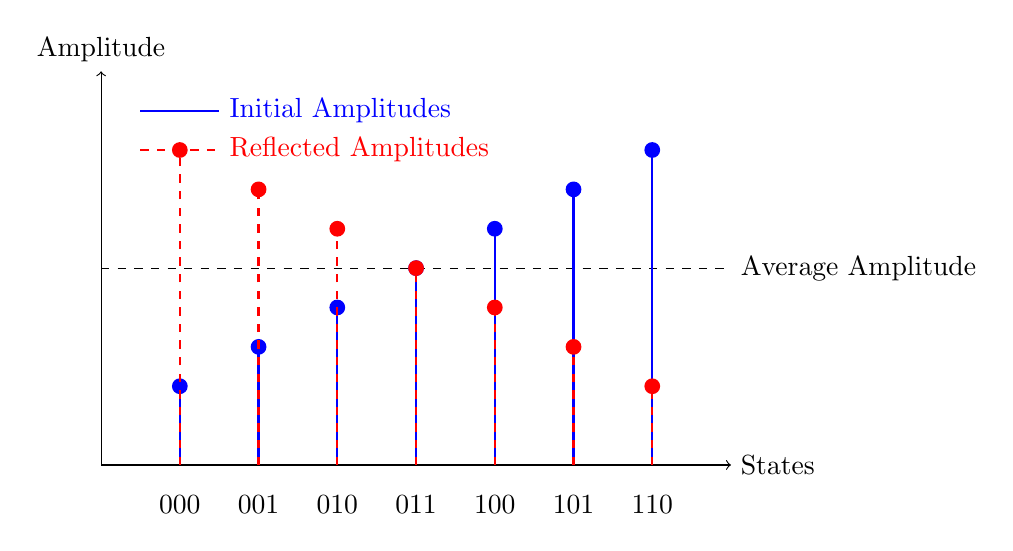
\begin{tikzpicture}
  % Draw axes
  \draw[->] (0,0) -- (8,0) node[right]{States};
  \draw[->] (0,0) -- (0,5) node[above]{Amplitude};

  % Draw average amplitude line
  \draw[dashed] (0,2.5) -- (8,2.5) node[right]{Average Amplitude};

  % Draw initial amplitudes
  \foreach \x/\y in {1/1, 2/1.5, 3/2, 4/2.5, 5/3, 6/3.5, 7/4} {
    \draw[blue, thick] (\x,0) -- (\x,\y);
    \fill[blue] (\x,\y) circle (0.1);
  }

  % Draw reflected amplitudes
  \foreach \x/\y in {1/4, 2/3.5, 3/3, 4/2.5, 5/2, 6/1.5, 7/1} {
    \draw[red, thick, dashed] (\x,0) -- (\x,\y);
    \fill[red] (\x,\y) circle (0.1);
  }

  % Labels
  \node at (1,-0.5) {\(\ket{000}\)};
  \node at (2,-0.5) {\(\ket{001}\)};
  \node at (3,-0.5) {\(\ket{010}\)};
  \node at (4,-0.5) {\(\ket{011}\)};
  \node at (5,-0.5) {\(\ket{100}\)};
  \node at (6,-0.5) {\(\ket{101}\)};
  \node at (7,-0.5) {\(\ket{110}\)};

  % Legend
  \draw[blue, thick] (0.5,4.5) -- (1.5,4.5) node[right]{Initial Amplitudes};
  \draw[red, thick, dashed] (0.5,4) -- (1.5,4) node[right]{Reflected Amplitudes};
\end{tikzpicture}
\end{center}

\vspace{0.3cm}

The blue bars represent the initial amplitudes of the states, and the red
dashed bars represent the amplitudes after inversion about the mean. The
marked state's amplitude is amplified, while the amplitudes of the other
states are reduced.


%%%%%%%%%%%%%%%%%%%%%%%%%%%%%%%%%%%%%%%%%%%%%%%%%%
% 2-Qubit Example
%%%%%%%%%%%%%%%%%%%%%%%%%%%%%%%%%%%%%%%%%%%%%%%%%%
\subsection*{2-Qubit Example}

To build intuition, consider the case \( n=2 \) (i.e., \( N=4 \)) with the winning
state chosen as \(\ket{11}\).

\vspace{0.3cm}

\textbf{Oracle:} For a 2-qubit system, the Oracle \(O\) can be implemented as a
controlled-\(Z\) (CZ) gate:
\[
  CZ =
  \begin{pmatrix}
    1 & 0 & 0 & 0 \\
    0 & 1 & 0 & 0 \\
    0 & 0 & 1 & 0 \\
    0 & 0 & 0 & -1
  \end{pmatrix},
\]

which multiplies the state \(\ket{11}\) by \(-1\).

\vspace{0.3cm}

\textbf{Diffusion Operator:} For 2 qubits, the diffusion operator is given by:

\[
  D = H^{\otimes 2}\; X^{\otimes 2}\; CZ\; X^{\otimes 2}\; H^{\otimes 2}.
\]

\vspace{0.3cm}

\textbf{2-Qubit Grover Circuit:}

\[
\begin{quantikz}
  \lstick{$\ket{0}$} & \gate{H} & \ctrl{1} & \gate{H} & \gate{X} & \qw & \ctrl{1} & \qw & \gate{X} & \gate{H} & \meter{} \\
  \lstick{$\ket{0}$} & \gate{H} & \ctrl{0} & \gate{H} & \gate{X} & \gate{H} & \gate{X} & \gate{H} & \gate{X} & \gate{H} & \meter{}
\end{quantikz}
\]

\vspace{0.3cm}

\noindent
\textbf{Explanation:}

\begin{itemize}
  \item \textbf{Oracle:} The Oracle adds a phase of \(-1\) to the winning
    state \(\ket{11}\), effectively marking it.
  \item \textbf{Diffusion Operator:} The diffusion circuit (implemented as
    \(H\;X\;CZ\;X\;H\)) reflects all amplitudes about the average. This
    inversion about the mean amplifies the amplitude of the marked state.
\end{itemize}

%%%%%%%%%%%%%%%%%%%%%%%%%%%%%%%%%%%%%%%%%%%%%%%%%%
% Algorithm Walkthrough and Pseudocode
%%%%%%%%%%%%%%%%%%%%%%%%%%%%%%%%%%%%%%%%%%%%%%%%%%

\index{Grover's Search Algorithm!pseudocode}
\subsection*{Walkthrough of the Algorithm and Generalization to \(n\) Qubits}

Grover's algorithm can be summarized in the following pseudocode:

\begin{algorithm}[H]
  \caption{Grover's Search Algorithm}
  \KwIn{A function \( f: \{0,1\}^n \rightarrow \{0,1\} \) with a unique
  marked state \( x_0 \) such that \( f(x_0) = 1 \).}
  \KwOut{The marked element \( x_0 \).}

  \textbf{Initialize:} Set the quantum state to \( \ket{\psi} \gets
  \ket{0}^{\otimes n} \).\\

  Apply \( H^{\otimes n} \) to obtain the uniform superposition:

  \[
    \ket{s} = H^{\otimes n}\ket{0}^{\otimes n} = \frac{1}{\sqrt{2^n}} \sum_{x
    \in \{0,1\}^n} \ket{x}.
  \]

  \For{\( i = 1 \) \KwTo \( \left\lfloor \frac{\pi}{4}\sqrt{2^n}
  \right\rfloor \)}{

    Apply the Oracle \( O \) which performs:

    \[
      O\ket{x} = (-1)^{f(x)}\ket{x},
    \]
    (i.e., flip the phase of the marked state).\;

    Apply the Diffusion Operator \( D = 2\ket{s}\bra{s} - I \)
    (which reflects amplitudes about the average).\;
  }

  Measure the state in the computational basis to obtain \( x_0 \).\;

\end{algorithm}

\vspace{0.3cm}

\noindent
\textbf{Detailed Explanation:}
\begin{enumerate}
  \item \textbf{Initialization:} All qubits are set to \(\ket{0}\) and then
    put into an equal superposition via \(H^{\otimes n}\).

  \item \textbf{Oracle Application:} The Oracle selectively flips the phase
    of the winning state(s) (e.g., for the marked state \(\ket{w}\),
    \(O\ket{w} = -\ket{w}\)).

  \item \textbf{Diffusion (Inversion about the Mean):} This operator reflects
    the state vector about the average amplitude. Geometrically, one can
    view the process as a rotation in a two-dimensional subspace.

  \item \textbf{Iteration:} Repeating the Oracle and Diffusion steps
    approximately \( \sqrt{2^n} \) times amplifies the probability amplitude of
    the marked state.

  \item \textbf{Measurement:} Finally, a measurement in the computational
    basis yields the marked element with high probability.
\end{enumerate}

This algorithm demonstrates how quantum algorithms can achieve a quadratic
speedup over classical brute-force search methods.

%%%%%%%%%%%%%%%%%%%%%%%%%%%%%%%%%%%%%%%%%%%%%%%%%%
% End of Lecture 9
%%%%%%%%%%%%%%%%%%%%%%%%%%%%%%%%%%%%%%%%%%%%%%%%%%
